\documentclass{article}

\usepackage{enumerate}
\usepackage{amssymb}
\usepackage{amsmath}
\usepackage{algorithm}
\usepackage{physics}
\usepackage{listings}
\usepackage[noend]{algpseudocode}
\usepackage{graphicx}

\graphicspath{ {./} }

\topmargin=-0.45in
\evensidemargin=0in
\oddsidemargin=0in
\textwidth=6.5in
\textheight=9.0in
\headsep=0.25in

\title{Chem 195: Problem Set 6}
\author{Michael Stephen Chen}


\begin{document}
\maketitle
\pagebreak

\textbf{NOTE:} The commented base simulation code is in the script \textit{h2o.m}. In \textit{ps6.m} I have a section for each problem that calls \textit{h2o.m}. Also all of the values presented are in atomic units.

\section*{Problem 1}
From the Hartree-Fock procedure, we find the energy of water in its equilibrium geometry to be $-71.677$ Hartrees.


\section*{Problem 2}
When we perform a Mulliken population analysis, we find that for each hydyogen atom, $q_H = -0.101$, and for the oxygen atom, $q_O = 0.201$. Our answer is not consistent with the general chemical intuition that electron density should be concentrated on the much more electronegative oxygen atom (and thus the oxygen should have a negative net effective charge while the hydrogens should have a net positive charge). The results of our HF simulation are the opposite of what we would expect.

\section*{Problem 3}
When we vary the OH bond length while keeping the other parameters constant we find $l_{OH}=2.0$ at our energetic minimum with a precision of 0.1.
\begin{center}
  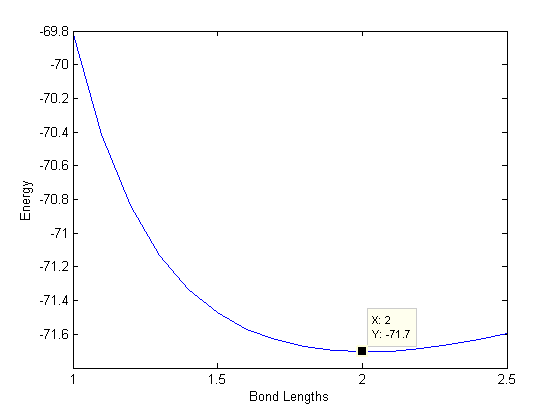
\includegraphics[scale=0.5]{prob3.png}
\end{center}


\section*{Problem 4}
When we vary the HOH bond angle while keeping the other parameters consistent we find that $\theta = 92$ degrees at the energetic minimum.
\begin{center}
  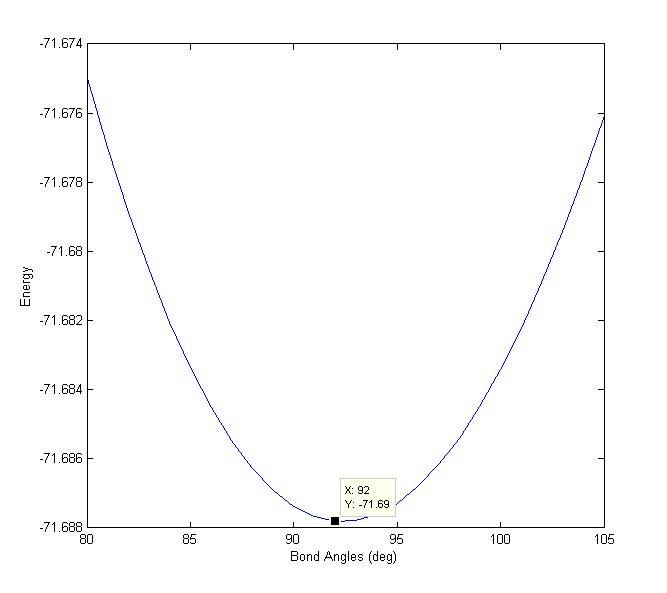
\includegraphics[scale=0.5]{prob4.png}
\end{center}


\section*{Problem 5}
When we on only vary one of the OH bond lengths we get the following plot of energy as a function of that one varying bond length.
\begin{center}
  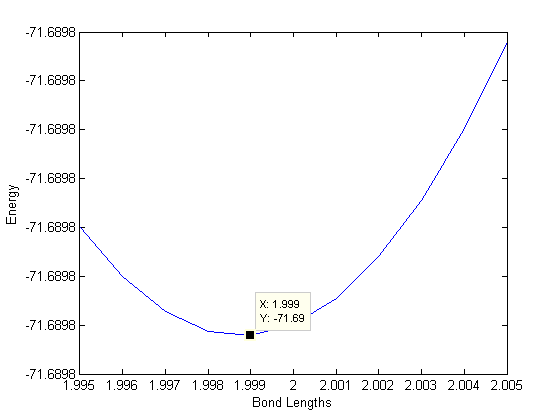
\includegraphics[scale=0.5]{prob5.png}
\end{center}


\section*{Problem 6}
Using our results from the previous problem we determine the curvature $d^2E/dR^2$ at the energy minimum. Our simulation's precision is $\delta=0.001$ and our energy minimum was $E(R)=-71.6898$ at $R=1.999$
\begin{align}
  \frac{d^2E}{dR^2} &= \frac{1}{\delta^2}[E(R+\delta) -2E(R) + E(R-\delta)]\\
  &= 0.624372
\end{align}


\section*{Problem 7}
To determine the excitation energy of for OH stretching we note that $\hbar$, and the electron mass $m_e$ are unity in atomic units. Since we are working in atomic units, we estimate the mass of hydrogen and oxygen as, respectively, 1 and 8 times the proton-electron mass ratio (1836.153). We also recall that the effective mass for a two body oscillator is:
$$\mu = \frac{m_1*m_2}{m_1+m_2}$$
Where $m_1$ is the mass of one H and $m_2$ is the mass of OH. To find the stretch energy in wavenumbers:
\begin{align}
  \hbar\omega_{OH} &= \sqrt{m^{-1}d^2E/dR^2} \times \frac{2.2\times 10^5 cm^{-1}}{1 hartree}\\
  &= 4276.305 cm^{-1}
\end{align}
Our result is considerably larger (around 10\%) than the known OH stretch energies for water ($3657 cm^{-1}$ and $3756 cm^{-1}$ for symmetric and antisymmetric water stretches)


\section*{Problem 8}
From our calculations we found the eigenvalues of the Fock matrix to be
\begin{center}
  $\begin{array}{c}
    Fock Eigs \\ \hline
    -20.0592 \\
    -1.3314 \\
    -0.5472 \\
    -0.3485 \\
    -0.1770 \\
    0.7204 \\
    0.8692 \\
  \end{array}$
\end{center}

To estimate the energy of the first ionization we apply Koopman's theorem where $N$ is the number of electrons. $\epsilon_{\mu}$ is the highest eigenvalue of the Fock matrix corresponding to the highest energy occupied orbital, which in this case is the 5th highest energy orbital given that $N=10$ and we can fit 2 electrons per orbital.
$$E_{HOH}(N+1) - E_{HOH}(N) = -\epsilon_{\mu} = 0.1770 Hartrees$$

Generally we see that decreasing the bond angle increases the first ionization potential estimate, and vice-versa, while lowering the bond lengths decreases the ionization potentials
\begin{center}
  $\begin{array}{c|c}
    \theta & Ionization Potential \\ \hline
    95 & 0.1798 \\
    100 & 0.1785 \\
    104.52 & 0.1770 \\
    110 & 0.1747 \\
    115 & 0.1722 
  \end{array}$
\end{center}

\begin{center}
  $\begin{array}{c|c}
    Bond Lengths & Ionization Potential \\ \hline
    1.75 & 0.1738 \\
    1.809 & 0.1770 \\
    1.85 & 0.1796
  \end{array}$
\end{center}


\end{document}
